%settings
\setlength{\parindent}{2ex}
\phantomsection
%text
%--------------------------------------Task1----------------------------------
\section{Model of the application and Use Case Diagrams.}
\begin{figure}[h!]
	\centering
	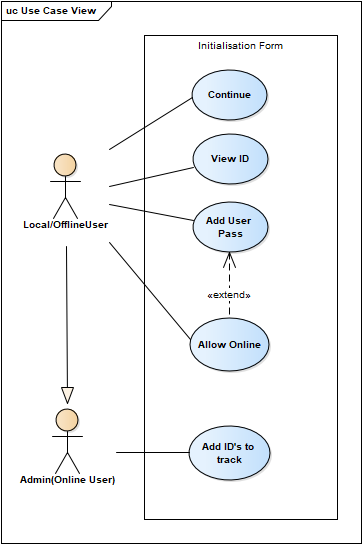
\includegraphics[keepaspectratio=true,scale=0.7]{U1}
	\caption{Initialization Form.} 
\end{figure}
\begin{flushleft}
\begin{enumerate}
		\item[•] My application has 2 types of actors \textbf{Local} which works in offline mode as well and \textbf{Admin} which is a generalized form of a Local User.
    	\item[•] A Local User can become an Admin after choosing the \textbf{Allow Online} option.
    	\item[•] \textbf{Allow Online} can be only accessed after inputting a \textbf{User Pass}. 
    	\item[•] An Admin has the option to add Local Users who he could track data.
      	\item[•] In order to add a Local User the admin has to input their ID and their User Pass.
    	\item[•] Upon initializing the application each Local User is given an ID. 
    	\item[•] All types of Users/actors must press continue to go to selection form.
\end{enumerate}
\end{flushleft}

\newpage \begin{figure}[h!]
	\centering
	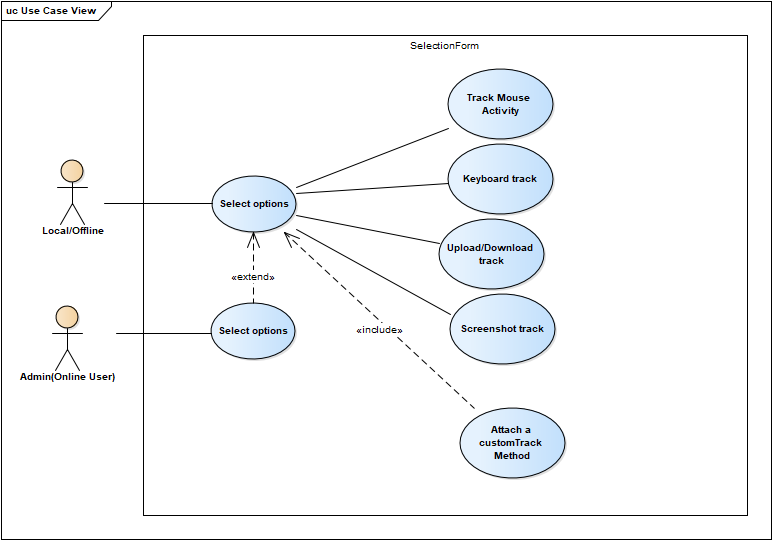
\includegraphics[keepaspectratio=true,width=\textwidth]{U2}
	\caption{Selection Form.} 
\end{figure}
\begin{flushleft}
\begin{enumerate}
		\item[•] After completing the initialization form, the Local/Offline User can Select Options from Default Tracking Methods \textit{(Keyboard Track,Track Mouse Activity,Upload/Download Track,Screenshot Track)}.
		\item[•] Additionally a Local user can add their own Tracking Method, by selecting \textbf{Attach a custom Track Method}.
		\item[•] If a Local user is a part of a network where there is an Admin then the Select Options that he has made will be overwritten by the Select Options that the Admin has on his machine.
\end{enumerate}
\end{flushleft}

\newpage \begin{figure}[h!]
	\centering
	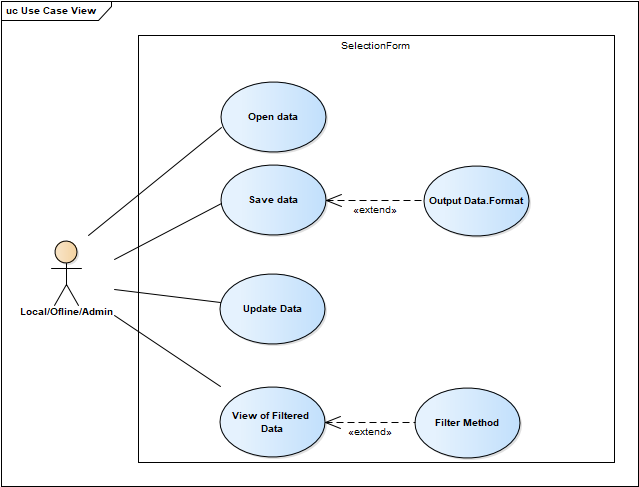
\includegraphics[keepaspectratio=true,width=\textwidth]{U3}
	\caption{Output Form.} 
\end{figure}
\begin{flushleft}
After completing the \textbf{Selection Form}, the Actor which in this case represents all types of users has 3 options to chose to get the data that was tracked.
\begin{enumerate}
		\item[•] He can View the data that was tracked and update it by pressing Update Data button and apply filtering methods to View the data.
		\item[•] Or he can save the data that was tracked;If a filtering method was used then data outputted will be influenced by the filter. 
		\item[•] Or he can open and view a data that was saved before.
\end{enumerate}
\end{flushleft}
%--------------------------------------Task2----------------------------------
\newpage
\section{Basic and alternate flows of use cases.}
\begin{flushleft}
\textbf{Initialization Form.}\par
Basic flow.(Offline)\par
\begin{enumerate}
		\item[•] Local/Offline user is given ID.
    	\item[•] Press Continue
\end{enumerate}
Alternate flow.(Local)\par
\begin{enumerate}
		\item[•] Local/Offline user is given ID.
    	\item[•] Input User Pass and check Allow online
    	\item[•] Press Continue
\end{enumerate}
Alternate flow.(Admin)\par
\begin{enumerate}
		\item[•] Local/Offline user is given ID.
    	\item[•] Input User Pass and check Allow online
    	\item[•] Add ID and User Pass.(How many Admin desires)
    	\item[•] Press Continue
\end{enumerate}

\textbf{Selection Form.}\par
Basic flow.(Local/Offline)\par
\begin{enumerate}
		\item[•] Local/Offline user Selects the tracking methods.
\end{enumerate}
Alternate flow.(Local/Offline)\par
\begin{enumerate}
    	\item[•] Local/Offline user adds a new tracking method.
    	\item[•] Local/Offline user selects the tracking methods.
\end{enumerate}
Alternate flow.(Admin)\par
\begin{enumerate}
		\item[•] Admin user selects the tracking methods.
    	\item[•] Local/Offline user selections get overwritten.
\end{enumerate}
%--------------------------------------------here!!!!!!!!!!!!!!!!!!!!!!!!!!!!!!!!!!!!
\newpage\textbf{Output Form.}\par
Basic flow.\par
\begin{enumerate}
        \item[•] User presses Update.
		\item[•] User Views the data.
		\item[•] User Saves the data.
\end{enumerate}
Alternate flow.\par
\begin{enumerate}
    	\item[•] User filters the data.
    	\item[•] User presses Update.
    	\item[•] User views filtered data.
    	\item[•] User Saves the data.
\end{enumerate}
Alternate flow.\par
\begin{enumerate}
		\item[•] User opens a data file.
    	\item[•] User Views the data.
    	\item[•] User filters the data.
    	\item[•] User presses Update.
    	\item[•] User views filtered data.
    	\item[•] User Saves the data. 
\end{enumerate}
\end{flushleft}
\clearpage
